% ============================================================
% Chapter 9: Hilbert's Problem 8 — The Goldbach Conjecture
% ============================================================

\chapter{The Goldbach Conjecture}

\begin{unsolvedbox}
The Goldbach Conjecture (binary version) is \textbf{unsolved}. It has been verified computationally for all even integers up to $4 \times 10^{18}$, and the related ternary version was proved by Helfgott in 2013, but no general proof of the binary conjecture is known.
\end{unsolvedbox}

% ------------------------------------------------------------
\begin{figure}[htbp]
\centering
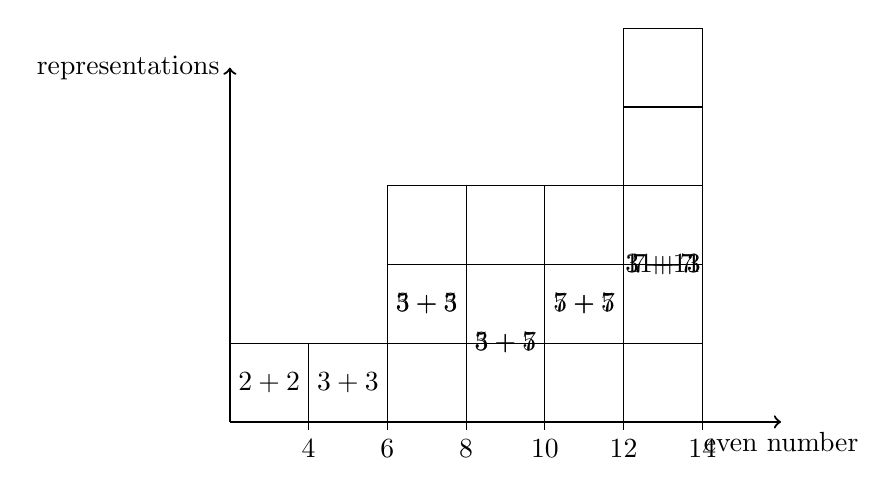
\begin{tikzpicture}
  \draw[thick,->] (0,0) -- (7,0) node[below] {even number};
  \draw[thick,->] (0,0) -- (0,4.5) node[left] {representations};
  \foreach \x/\lbl in {1/4,2/6,3/8,4/10,5/12,6/14}
    \draw (\x,0.1) -- (\x,-0.1) node[below] {$\lbl$};
  \draw (0,0) rectangle (1,1);
  \node at (0.5,0.5) {$2+2$};
  \draw (1,0) rectangle (2,1);
  \node at (1.5,0.5) {$3+3$};
  \draw (2,0) rectangle (3,3);
  \node at (2.5,1.5) {$3+5$};
  \draw (2,1) rectangle (3,2);
  \node at (2.5,1.5) {$5+3$};
  \draw (3,0) rectangle (4,2);
  \node at (3.5,1) {$3+7$};
  \draw (3,1) rectangle (4,2);
  \node at (3.5,1) {$5+5$};
  \draw (3,2) rectangle (4,3);
  \draw (4,0) rectangle (5,3);
  \node at (4.5,1.5) {$5+7$};
  \draw (4,1) rectangle (5,3);
  \node at (4.5,1.5) {$7+5$};
  \draw (4,2) rectangle (5,3);
  \draw (5,0) rectangle (6,4);
  \node at (5.5,2) {$3+11$};
  \draw (5,1) rectangle (6,4);
  \node at (5.5,2) {$7+7$};
  \draw (5,2) rectangle (6,4);
  \draw (5,3) rectangle (6,4);
  \node at (5.5,2) {$11+3$};
  \draw (5,4) rectangle (6,5);
\end{tikzpicture}
\caption{Goldbach representations for small even numbers. Each bar shows the number of ways to write the even number as a sum of two primes. For example, $10 = 3+7 = 5+5$ has two representations.}
\label{fig:goldbach}
\end{figure}

\section{Historical Context}
% ------------------------------------------------------------

The story of the Goldbach Conjecture begins not in a lecture hall or a journal, but in a letter. In 1742, the Prussian mathematician Christian Goldbach (1690--1764) wrote to Leonhard Euler, then the most prominent mathematician in Europe, with a simple but tantalizing observation. Goldbach noticed that many even numbers can be written as the sum of two prime numbers. For instance:
\[
    4 = 2 + 2, \quad 6 = 3 + 3, \quad 8 = 3 + 5, \quad 10 = 3 + 7 = 5 + 5.
\]
Goldbach proposed that \emph{every} even integer greater than 2 has this property. Euler replied that he believed the conjecture to be true but was unable to prove it. Thus began one of the oldest and most famous open problems in number theory.

The problem is remarkable for its simplicity. Anyone who understands what a prime number is can state the conjecture, and yet nearly three centuries of effort have failed to produce a proof. It is a humbling reminder that the distribution of prime numbers---the ``atoms'' of arithmetic---remains deeply mysterious.

\subsection{The Distribution of Primes}

To understand why the Goldbach Conjecture is so difficult, we need to understand what is and is not known about the distribution of prime numbers.

A \textbf{prime number} is an integer $p > 1$ whose only positive divisors are $1$ and $p$ itself. The first few primes are:
\[
    2,\ 3,\ 5,\ 7,\ 11,\ 13,\ 17,\ 19,\ 23,\ 29,\ 31,\ \ldots
\]
Primes become sparser as we look at larger numbers, but they never stop appearing---Euclid proved this over two thousand years ago. The fundamental question is: \emph{how} sparse?

The \textbf{prime-counting function} $\pi(x)$ counts the number of primes less than or equal to $x$. Gauss and Legendre, in the late eighteenth century, conjectured on the basis of numerical evidence that $\pi(x)$ grows approximately like $x / \ln x$. This conjecture was eventually proved and refined into one of the crowning achievements of nineteenth-century mathematics.

\begin{theorem}[Prime Number Theorem]
\label{thm:pnt}
As $x \to \infty$,
\[
    \pi(x) \sim \frac{x}{\ln x}.
\]
Equivalently, $\pi(x) \sim \operatorname{Li}(x)$, where $\operatorname{Li}(x) = \int_2^x \frac{dt}{\ln t}$ is the \emph{logarithmic integral}, a somewhat better approximation.
\end{theorem}

The Prime Number Theorem was proved independently by Jacques Hadamard and Charles-Jean de la Vall\'ee Poussin in 1896, using deep methods from complex analysis. Their proofs relied on the fact that the Riemann zeta function $\zeta(s) = \sum_{n=1}^{\infty} n^{-s}$ has no zeros on the line $\Re(s) = 1$ in the complex plane. (This is a weaker statement than the famous Riemann Hypothesis, which asserts that \emph{all} nontrivial zeros lie on the line $\Re(s) = \tfrac{1}{2}$.)

The Prime Number Theorem tells us that a ``random'' large integer $n$ has probability approximately $1/\ln n$ of being prime. This heuristic is the starting point for understanding Goldbach's Conjecture.

% ------------------------------------------------------------
\section{The Problem}
% ------------------------------------------------------------

\begin{problem_statement}[Goldbach's Conjecture, 1742]
Every even integer $n > 2$ can be expressed as the sum of two primes. That is, for every even $n > 2$, there exist primes $p$ and $q$ such that
\[
    n = p + q.
\]
\end{problem_statement}

This is sometimes called the \textbf{binary} Goldbach Conjecture (because it involves two summands) or the \textbf{strong} Goldbach Conjecture. It should be distinguished from the following weaker statement:

\begin{problem_statement}[Ternary Goldbach Conjecture]
Every odd integer $n > 5$ can be expressed as the sum of three primes. That is, for every odd $n > 5$, there exist primes $p$, $q$, and $r$ such that
\[
    n = p + q + r.
\]
\end{problem_statement}

The ternary conjecture is ``weaker'' in the sense that it follows from the binary conjecture: if $n > 5$ is odd, then $n - 3 > 2$ is even, and if the binary conjecture holds, we can write $n - 3 = p + q$, so $n = 3 + p + q$ is a sum of three primes. Conversely, the ternary conjecture does \emph{not} imply the binary conjecture, so proving the ternary case is easier.

\subsection{Computational Evidence}

The Goldbach Conjecture has been verified by computer for all even integers up to $4 \times 10^{18}$---a staggering $4$ quintillion. This verification was carried out by Oliveira e Silva, Sa da Fonseca, and others using distributed computing. The conjecture holds without exception.

But as Hardy and Littlewood were fond of emphasizing, numerical verification is not proof. The history of number theory is littered with conjectures that held for millions of cases before failing. (For example, $\sum_{k=1}^{n} k^2 = n(n+1)(2n+1)/6$ holds for all $n$, but a similar-looking formula involving primes might fail only at astronomically large values.)

To appreciate the scale of the verification: the number $4 \times 10^{18}$ is roughly the number of grains of sand on Earth. The conjecture holds for every single one of them, and yet we cannot prove it.

% ------------------------------------------------------------
\section{Key Developments}
% ------------------------------------------------------------

The Goldbach Conjecture has resisted proof for nearly three centuries, but the effort has produced some of the most important tools in analytic number theory.

\subsection{The Hardy--Littlewood Circle Method}

The most powerful approach to the Goldbach Conjecture is the \textbf{circle method}, developed by G.\,H.\ Hardy and J.\,E.\ Littlewood in the 1920s. The idea is to translate the additive problem (``can $n$ be written as $p + q$?'') into a problem about complex analysis.

The starting point is a \emph{generating function}. For an even integer $n$, the number of ways to write $n = p + q$ with $p$ and $q$ prime is
\[
    R(n) = \sum_{\substack{p + q = n \\ p,\, q \text{ prime}}} 1.
\]
One can show using Fourier analysis that
\[
    R(n) = \int_0^1 \left( \sum_{p \leq N} e^{2\pi i p \alpha} \right)^2 e^{-2\pi i n \alpha} \, d\alpha,
\]
where the sum runs over primes $p$ up to some bound $N > n/2$, and $e(x) = e^{2\pi i x}$.

The integral is over the unit interval $[0,1]$, but it is dominated by contributions near \emph{rational} values of $\alpha$. Near $\alpha = 0$, the sum $\sum_p e(p\alpha)$ is large because the primes are ``in phase'' there. Near other rational points $a/q$ with small denominator $q$, the sum has predictable behavior given by the distribution of primes in arithmetic progressions. The remaining ``minor arcs''---the parts of $[0,1]$ not close to any rational with small denominator---contribute a smaller error.

By carefully estimating the contribution from the major arcs and bounding the contribution from the minor arcs, Hardy and Littlewood obtained a formula for $R(n)$ of the form
\[
    R(n) \sim \mathfrak{S}(n) \cdot \frac{n}{(\ln n)^2} \cdot C,
\]
where $\mathfrak{S}(n)$ is the \textbf{Goldbach singular series} and $C$ is a positive constant. The singular series encodes the local constraints imposed by divisibility by small primes:
\[
    \mathfrak{S}(n) = 2 \prod_{p > 2} \left( 1 - \frac{1}{(p-1)^2} \right) \prod_{\substack{p \mid n \\ p > 2}} \frac{p - 1}{p - 2}.
\]
This product converges to a positive constant, so the heuristic prediction is that $R(n) \to \infty$ as $n \to \infty$---in fact, $R(n)$ grows roughly like $n / (\ln n)^2$. The conjecture, in other words, should be ``true with room to spare.''

\subsection{Vinogradov's Theorem (1937)}

The first major result using the circle method came from the Soviet mathematician Ivan Vinogradov (1891--1983). In 1937, he proved:

\begin{theorem}[Vinogradov, 1937]
Every sufficiently large odd integer is the sum of three primes.
\end{theorem}

``Sufficiently large'' here means that there exists some constant $N_0$ such that every odd $n > N_0$ works. Vinogradov's proof did not specify a value for $N_0$, and it was far too large to be checked computationally. The ternary Goldbach Conjecture for smaller odd numbers remained open for decades.

Vinogradov's method was a tour de force of analytic number theory. He refined the circle method to handle the error terms that arise when approximating sums over primes by integrals, using deep estimates for exponential sums over primes. His work established the circle method as the central tool in additive number theory and influenced generations of mathematicians.

\subsection{Chen's Theorem (1973)}

The closest result to the binary Goldbach Conjecture is due to the Chinese mathematician Chen Jingrun (1933--2001):

\begin{theorem}[Chen, 1973]
Every sufficiently large even integer is the sum of a prime and a \emph{semiprime}---that is, a product of at most two primes.
\end{theorem}

More precisely, Chen proved that every sufficiently large even integer can be written as
\[
    n = p + q \quad \text{or} \quad n = p + q_1 q_2,
\]
where $p$, $q$, $q_1$, $q_2$ are all prime.

This is tantalizingly close to the Goldbach Conjecture. The only ``defect'' is that one of the summands might be a product of two primes instead of a single prime. To see why this is ``almost'' the conjecture: if you write $n = p + q_1 q_2$, then you need only show that one of the $q_i$ equals 1 to get a Goldbach representation---but of course 1 is not prime, so this doesn't quite work.

Chen's theorem is the strongest result of its kind, and despite decades of effort, nobody has been able to close the gap. The difficulty lies in the fundamental limitation of the circle method when applied to two variables: the minor arc estimates are not strong enough to force both summands to be prime.

\subsection{Helfgott's Proof of the Ternary Conjecture (2013)}

The ternary Goldbach Conjecture was the subject of a remarkable proof by the Peruvian--French mathematician Harald Helfgott. Building on work by Vinogradov, Montgomery, and Vaughan, Helfgott completed the proof in two stages:

\begin{enumerate}
    \item \textbf{Large values (2013):} Helfgott proved that every odd $n > 10^{29}$ is the sum of three primes, making explicit the implicit constant in Vinogradov's theorem. His method used refined estimates for the circle method and computer-assisted verification of certain bounds.
    \item \textbf{Small values (2013):} Together with David Platt, Helfgott used computer verification to check the ternary Goldbach Conjecture for all odd $n$ up to $10^{29}$.
\end{enumerate}

\begin{theorem}[Helfgott, 2013]
Every odd integer $n > 5$ is the sum of three primes.
\end{theorem}

Helfgott's proof is notable not only for its mathematical content but also for its methodology. The proof combines traditional analytic arguments with extensive computer verification---a ``proof by calculation'' for the small cases, and a ``proof by analysis'' for the large ones. The computer-assisted parts have been independently verified using the Coq proof assistant, giving the result an extraordinary level of certainty.

The ternary Goldbach Conjecture is therefore \emph{solved}. But the binary Goldbach Conjecture---the original problem posed by Goldbach---remains wide open.

% ------------------------------------------------------------
\section{Current Status: Unsolved}
% ------------------------------------------------------------

The binary Goldbach Conjecture remains one of the most famous unsolved problems in mathematics. As of this writing:

\begin{itemize}
    \item The conjecture has been verified computationally for all even integers up to $4 \times 10^{18}$, with no counterexample found.
    \item Chen's theorem (1973) gets ``almost'' there: every sufficiently large even number is a prime plus a semiprime.
    \item The ternary Goldbach Conjecture was proved by Helfgott (2013), but this does not resolve the binary case.
    \item No proof strategy is known that would definitively settle the conjecture.
\end{itemize}

The difficulty is fundamentally about the limitations of current analytic methods. The circle method works beautifully for three or more variables, where the major arcs dominate and the error terms can be controlled. But for two variables, the minor arcs contribute too much, and the method falls short. New ideas---perhaps from additive combinatorics, the theory of exponential sums, or entirely new directions---may be needed.

\subsection{Related Conjectures}

The Goldbach Conjecture belongs to a rich family of conjectures about additive properties of primes:

\begin{itemize}
    \item \textbf{The Twin Prime Conjecture.} There are infinitely many pairs of primes $(p, p+2)$---twin primes. This is closely related to Goldbach: twin primes are primes with the smallest possible gap, while Goldbach representations involve two primes with a gap of exactly $n - 2p$.

    \item \textbf{Legendre's Conjecture.} For every positive integer $n$, there is at least one prime between $n^2$ and $(n+1)^2$. This is about the local distribution of primes, while Goldbach is about their additive structure.

    \item \textbf{Polignac's Conjecture (1849).} For every even positive integer $2k$, there are infinitely many pairs of primes $(p, p + 2k)$. The Twin Prime Conjecture is the special case $k = 1$.

    \item \textbf{The $n$th Prime Gap.} Understanding how large the gap $p_{n+1} - p_n$ can be is related to understanding how ``evenly'' primes are distributed, which is relevant to Goldbach representations.
\end{itemize}

These conjectures are all interconnected. Progress on any one of them often sheds light on the others, and they share the common theme of understanding the \emph{additive} structure of the primes---as opposed to their multiplicative structure, which is better understood.

% ------------------------------------------------------------
\section*{Common Questions}
% ------------------------------------------------------------

\begin{description}[font=\bfseries, leftmargin=2em, style=nextline]

\item[Q: If the conjecture has been verified up to $4 \times 10^{18}$, why isn't that a proof?]\hfill\\
No amount of checking finite cases can prove a statement about \emph{all} even numbers. There are infinitely many even integers, and the verification, while covering a staggering range, only touches a vanishingly small fraction of them. History provides cautionary tales: the conjecture that $\pi(x) < \operatorname{Li}(x)$ (the prime-counting function is always less than the logarithmic integral) holds for all $x$ up to about $10^{316}$, yet it eventually fails. A billion cases might seem convincing, but mathematics demands a logically airtight argument, not statistical evidence.

\item[Q: What's the difference between the weak (ternary) and strong (binary) Goldbach conjectures?]\hfill\\
The \textbf{strong (binary)} conjecture states that every even $n > 2$ is the sum of \emph{two} primes. The \textbf{weak (ternary)} conjecture states that every odd $n > 5$ is the sum of \emph{three} primes. The ternary is called ``weaker'' because it follows from the binary: if $n > 5$ is odd, then $n-3$ is even and $>2$, and if the binary conjecture holds, $n-3 = p+q$, so $n = 3+p+q$ is a sum of three primes. The reverse is not true. Helfgott proved the ternary conjecture in 2013, but the binary conjecture remains open.

\item[Q: Why is the circle method called that? Do you actually draw circles?]\hfill\\
Yes, in a literal sense. The Hardy--Littlewood circle method works by representing the number of Goldbach representations as a complex contour integral over the unit circle $|z| = 1$ (or equivalently $\alpha \in [0,1]$ via $z = e^{2\pi i \alpha}$). The integral is then split into ``major arcs'' (small intervals around rational numbers with small denominators, where the behavior is predictable) and ``minor arcs'' (the rest, where cancellations occur). The name comes from this geometric picture of dividing the circle into arcs of two types. The method has become a cornerstone of analytic number theory, used on problems far beyond Goldbach.

\item[Q: Why is the Goldbach conjecture so hard to prove if it's been checked for quintillions of numbers?]\hfill\\
The difficulty is that primes are defined multiplicatively (by their divisors), but Goldbach is an \emph{additive} problem. There is no simple formula linking the multiplicative structure of a number with how it behaves in sums. The best available tools---the circle method, sieve methods---give approximate answers but not exact ones. For the binary case, the error terms in the estimates are just barely too large to force the conclusion. Improving them by even a tiny amount would require a fundamentally new idea rather than a refinement of existing techniques.

\item[Q: Does $1$ count as a prime for Goldbach's conjecture?]\hfill\\
No. The Goldbach conjecture uses the modern definition of primes: an integer $p > 1$ whose only positive divisors are $1$ and itself. The number $1$ is not prime (it is a unit). If $1$ were counted, the conjecture would be trivially true in a different sense (every even $n = 1 + (n-1)$), but that is not the intended problem. The conjecture is about the distribution of genuine primes, and $1$ is excluded by convention.

\item[Q: What does Chen's theorem actually say, and why is it the closest result?]\hfill\\
Chen's theorem (1973) states that every sufficiently large even integer is the sum of a prime and a number that is either prime or a product of two primes (a \emph{semiprime}). In symbols, $n = p + q$ where $p$ is prime and $q$ is either prime or $q = q_1 q_2$ with $q_1, q_2$ prime. This is tantalizingly close to Goldbach: the only ``defect'' is that one term might be a product of two primes instead of a single prime. More than fifty years later, nobody has been able to eliminate this possibility. The result represents the limit of what sieve methods can achieve for the binary problem.

\item[Q: Are there any prizes for proving the Goldbach conjecture?]\hfill\\
Unlike the Riemann Hypothesis or the Poincaré Conjecture, the Goldbach conjecture does not have a Clay Millennium Prize ($1$ million). However, it is widely considered one of the most famous unsolved problems in mathematics, and proving it would bring immense recognition and likely several major prizes (Fields Medal, Abel Prize, etc.). There is also a standing offer of \$1 million from a private publisher (Faber and Faber) that was announced in 2000, though its terms are somewhat unusual and time-limited. The real reward would be the mathematical insight needed to crack the problem, which would almost certainly revolutionize our understanding of prime numbers.

\end{description}

% ------------------------------------------------------------
\section{Exercises}
% ------------------------------------------------------------

\begin{enumerate}

    \item \textbf{Verifying Goldbach for small numbers.}
    \begin{enumerate}
        \item Express each even integer from $4$ to $30$ as a sum of two primes. In how many ways can each number be expressed?
        \item Find an even integer that can be expressed as a sum of two primes in at least $5$ different ways.
        \item Does the number of Goldbach representations appear to increase with $n$? Explain informally why you might expect this.
    \end{enumerate}

    \item \textbf{Goldbach representations.}
    \begin{enumerate}
        \item Let $r(n)$ denote the number of ways to write $n = p + q$ where $p$ and $q$ are prime and $p \leq q$. Compute $r(n)$ for $n = 10, 12, 14, 16, 18, 20$.
        \item The Hardy--Littlewood formula predicts that $r(n) \sim C \cdot n / (\ln n)^2$ for some constant $C > 0$. Using your values from part (a), estimate the ratio $r(n) \cdot (\ln n)^2 / n$. Does this ratio appear to stabilize?
    \end{enumerate}

    \item \textbf{The Prime Number Theorem.}
    \begin{enumerate}
        \item Using the Prime Number Theorem, estimate the probability that a random even integer near $n$ is the sum of two primes. (\emph{Hint:} If $n$ is fixed and $p$ is a ``random'' prime near $n/2$, what is the probability that $n - p$ is also prime? How many choices of $p$ are there?)
        \item Explain informally why the Hardy--Littlewood heuristic predicts $r(n) \sim C \cdot n / (\ln n)^2$, rather than, say, $C / \ln n$ or $C \cdot (\ln n)^2$.
    \end{enumerate}

    \item \textbf{Chen's Theorem.}
    \begin{enumerate}
        \item Find an even integer $n \geq 30$ that can be written as $n = p + q$ with $p$ prime and $q$ either prime or a product of exactly two primes, but \emph{not} as $n = p + q$ with both $p$ and $q$ prime. (That is, find a number that ``needs'' Chen's generalization.)
        \item Explain in your own words why Chen's theorem is ``almost'' the Goldbach Conjecture but not quite.
    \end{enumerate}

    \item \textbf{Why is the binary case harder?}
    The ternary Goldbach Conjecture was proved in 2013, but the binary case remains open. In one or two paragraphs, explain at an intuitive level why adding a third prime makes the problem easier. (\emph{Hint:} Think about how many ``degrees of freedom'' you have. With three primes, you have more room to maneuver; with two, every prime in the sum is constrained.)

    \item[$\star$] \textbf{The Goldbach Comet.} Plot the number of Goldbach representations $r(n)$ for even $n$ from $4$ to $200$. You should observe a characteristic ``comet'' shape: the values cluster along several curved bands. Explain informally why this structure arises. (\emph{Hint:} Consider what happens when $n$ is divisible by 3 versus when it is not.)

\end{enumerate}
